\documentclass[a4paper]{article}
\usepackage{geometry}
\usepackage{graphicx}
\usepackage{natbib}
\usepackage{amsmath}
\usepackage{amssymb}
\usepackage{amsthm}
\usepackage{paralist}
\usepackage{epstopdf}
\usepackage{tabularx}
\usepackage{longtable}
\usepackage{multirow}
\usepackage{multicol}
\usepackage[hidelinks]{hyperref}
\usepackage{fancyvrb}
\usepackage{algorithm}
\usepackage{algorithmic}
\usepackage{float}
\usepackage{paralist}
\usepackage[svgname]{xcolor}
\usepackage{enumerate}
\usepackage{array}
\usepackage{times}
\usepackage{url}
\usepackage{fancyhdr}
\usepackage{comment}
\usepackage{environ}
\usepackage{times}
\usepackage{textcomp}
\usepackage{caption}
\usepackage{color}
\usepackage{xcolor}

\urlstyle{rm}

\setlength\parindent{0pt} % Removes all indentation from paragraphs
\theoremstyle{definition}
\newtheorem{definition}{Definition}[]
\newtheorem{conjecture}{Conjecture}[]
\newtheorem{example}{Example}[]
\newtheorem{theorem}{Theorem}[]
\newtheorem{lemma}{Lemma}
\newtheorem{proposition}{Proposition}
\newtheorem{corollary}{Corollary}

\floatname{algorithm}{Procedure}
\renewcommand{\algorithmicrequire}{\textbf{Input:}}
\renewcommand{\algorithmicensure}{\textbf{Output:}}
\newcommand{\abs}[1]{\lvert#1\rvert}
\newcommand{\norm}[1]{\lVert#1\rVert}
\newcommand{\RR}{\mathbb{R}}
\newcommand{\CC}{\mathbb{C}}
\newcommand{\Nat}{\mathbb{N}}
\newcommand{\br}[1]{\{#1\}}
\DeclareMathOperator*{\argmin}{arg\,min}
\DeclareMathOperator*{\argmax}{arg\,max}
\renewcommand{\qedsymbol}{$\blacksquare$}

\definecolor{dkgreen}{rgb}{0,0.6,0}
\definecolor{gray}{rgb}{0.5,0.5,0.5}
\definecolor{mauve}{rgb}{0.58,0,0.82}

\newcommand{\Var}{\mathrm{Var}}
\newcommand{\Cov}{\mathrm{Cov}}

\newcommand{\vc}[1]{\boldsymbol{#1}}
\newcommand{\xv}{\vc{x}}
\newcommand{\Sigmav}{\vc{\Sigma}}
\newcommand{\alphav}{\vc{\alpha}}
\newcommand{\muv}{\vc{\mu}}

\newcommand{\red}[1]{\textcolor{red}{#1}}

\def\x{\mathbf x}
\def\y{\mathbf y}
\def\w{\mathbf w}
\def\v{\mathbf v}
\def\E{\mathbb E}
\def\V{\mathbb V}

% TO SHOW SOLUTIONS, include following (else comment out):
\newenvironment{soln}{
    \leavevmode\color{blue}\ignorespaces
}{}


\hypersetup{
%    colorlinks,
    linkcolor={red!50!black},
    citecolor={blue!50!black},
    urlcolor={blue!80!black}
}

\geometry{
  top=1in,            % <-- you want to adjust this
  inner=1in,
  outer=1in,
  bottom=1in,
  headheight=3em,       % <-- and this
  headsep=2em,          % <-- and this
  footskip=3em,
}


\pagestyle{fancyplain}
\lhead{\fancyplain{}{Homework 2}}
\rhead{\fancyplain{}{CS 760 Machine Learning}}
\cfoot{\thepage}

\title{\textsc{Homework 2}} % Title

%%% NOTE:  Replace 'NAME HERE' etc., and delete any "\red{}" wrappers (so it won't show up as red)

\author{
\red{$>>$Guruprasad Viswanathan Ramesh$<<$} \\
\red{$>>$9082378762$<<$}\\
} 

\date{}

\begin{document}

\maketitle 


\textbf{Instructions:} 
Use this latex file as a template to develop your homework. Submit your homework on time as a single pdf file to Canvas. Please wrap your code and upload to a public GitHub repo, then attach the link below the instructions so that we can access it. You can choose any programming language (i.e. python, R, or MATLAB), as long as you implement the algorithm from scratch (e.g. do not use sklearn on questions 1 to 7 in section 2). Please check Piazza for updates about the homework.

\red{Github repo: https://github.com/Guruprasad68/CS760-Machine-Learrning-Spring2023}\\
\red{Note:Some figures appear in next pages. I have used reference to indicate which image belongs to which answer}
\section{A Simplified Decision Tree}
You are to implement a decision-tree learner for classification.
To simplify your work, this will not be a general purpose decision tree.  Instead, your program can assume that
\begin{itemize}
\item each item has two continuous features $\x \in \RR^2$
\item the class label is binary and encoded as $y \in \{0,1\}$
\item data files are in plaintext with one labeled item per line, separated by whitespace:
$$x_{11} \quad x_{12} \quad y_1$$
$$...$$
$$x_{n1} \quad x_{n2} \quad y_n$$
\end{itemize}

Your program should implement a decision tree learner according to the following guidelines:
\begin{itemize}
\item Candidate splits $(j,c)$ for numeric features should use a threshold $c$ in feature dimension $j$ in the form of $x_{\cdot j}\ge c$.
\item $c$ should be on values of that dimension present in the training data; i.e. the threshold is on training points, not in between training points. You may enumerate all features, and for each feature, use all possible values for that dimension.
\item You may skip those candidate splits with zero split information (i.e. the entropy of the split), and continue the enumeration.
\item The left branch of such a split is the ``then'' branch, and the right branch is ``else''.
\item Splits should be chosen using information gain ratio. If there is a tie you may break it arbitrarily.
\item The stopping criteria (for making a node into a leaf) are that 
	\begin{itemize}
	\item the node is empty, or
	\item all splits have zero gain ratio (if the entropy of the split is non-zero), or
	\item the entropy of any candidates split is zero
	\end{itemize}
\item To simplify, whenever there is no majority class in a leaf, let it predict $y=1$.
\end{itemize}

\section{Questions}
\begin{enumerate}
\item (Our algorithm stops at pure labels) [10 pts] If a node is not empty but contains training items with the same label, why is it guaranteed to become a leaf?  Explain. You may assume that the feature values of these items are not all the same. \\
\begin{soln}
    For the sake of explanation, let's assume that all the examples are labeled $'1'$. Let number of $'1'$ be $p$, number of $'0'$ be $n$, and total be $t$.
    Then the entropy at the node will be equal to $-(p/t*\log_{2}p/t + n/t*\log_{2}n/t)=-1log_21=0$ as $p=t$ and $n=0$ (our assumption). Further splitting will also lead to zero entropy. This means the node is without any 'impurity', and there can be no more effective information gain. Thus, this node is guaranteed to be a leaf node. 
\end{soln}

\item (Our algorithm is greedy)  [10 pts] Handcraft a small training set where both classes are present but the algorithm refuses to split; instead it makes the root a leaf and stop;
Importantly, if we were to manually force a split, the algorithm will happily continue splitting the data set further and produce a deeper tree with zero training error.
You should (1) plot your training set, (2) explain why.  Hint: you don't need more than a handful of items. \\
\begin{soln}
 Consider the following dataset in Figure \ref{fig:q2rootlead}:
    \begin{figure}[h!]
        \centering
        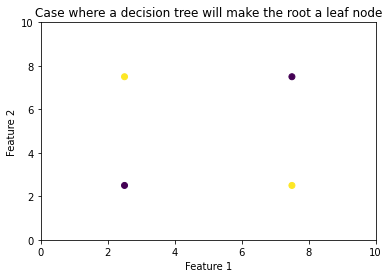
\includegraphics[width=0.5\textwidth]{images/q2_2_root_is_leaf.png}
        \caption{Dataset where a DT won't be able to make a split using a greedy algorithm}
        \label{fig:q2rootlead}
    \end{figure}

The reason why a node can't make a split is either if it is pure, which means it becomes a leaf, or if there is no information gain in splitting. Thus, the root can be the leaf node in a case where both positive and negative examples are present in the dataset when the information gain is zero for a split with either feature. Here in this dataset, the Information gain when the root is split across either feature 1 or feature 2 is zero. Thus, the root arbitrarily assigns a label and becomes the leaf.
\end{soln}

\item (Information gain ratio exercise)  [10 pts] Use the training set Druns.txt.  For the root node, list all candidate cuts and their information gain ratio. If the entropy of the candidate split is zero, please list its mutual information (i.e. information gain). Hint: to get $\log_2(x)$ when your programming language may be using a different base, use \verb|log(x)/log(2)|. Also, please follow the split rule in the first section. \\

\begin{soln}
The candidate cuts(feature index and the threshold), with it's information gain are as follows:
\begin{itemize}
    \item feature index: 0, Threshold: 0.0, Information Gain Ratio: 0
    \item feature index: 0, Threshold: 0.1, Information Gain Ratio: 0.10051807676021828
    \item feature index: 1, Threshold: -2.0, Information Gain Ratio: 0
    \item feature index: 1, Threshold: -1.0, Information Gain Ratio: 0.10051807676021828
    \item feature index: 1, Threshold: 0.0, Information Gain Ratio: 0.055953759631263845
    \item feature index: 1, Threshold: 1.0, Information Gain Ratio: 0.005780042205152189
    \item feature index: 1, Threshold: 2.0, Information Gain Ratio: 0.001144349517276632
    \item feature index: 1, Threshold: 3.0, Information Gain Ratio: 0.016411136842102134
    \item feature index: 1, Threshold: 4.0, Information Gain Ratio: 0.049749064181778435
     \item feature index: 1, Threshold: 5.0, Information Gain Ratio: 0.11124029586339801
     \item feature index: 1, Threshold: 6.0, Information Gain Ratio: 0.23609960614360798
     \item feature index: 1, Threshold: 7.0, Information Gain Ratio: 0.055953759631263845
     \item feature index: 1, Threshold: 8.0, Information Gain Ratio: 0.4301569161309807
\end{itemize}
    

\end{soln}
\item (The king of interpretability)  [10 pts] Decision tree is not the most accurate classifier in general.  However, it persists.  This is largely due to its rumored interpretability: a data scientist can easily explain a tree to a non-data scientist.  Build a tree from D3leaves.txt.  Then manually convert your tree to a set of logic rules.  Show the tree\footnote{When we say show the tree, we mean either the standard computer science tree view or some crude plaintext representation of the tree -- as long as you explain the format.  When we say visualize the tree, we mean a plot in the 2D $\x$ space that shows how the tree will classify any points.} and the rules. \\

\begin{soln}
    I used depth-first search with a pre-order traversal(root->left->right) for listing the nodes of the tree. The leaf node will be represented as 'Leaf Node' along with the label and the decision nodes will have the feature index and the threshold. The depth order traversal of the tree I obtained is as follows:\\
    Feature:0, Threshold:10\\
    Leaf Node---Label:1\\
    Feature:1, Threshold:3\\
    Leaf Node---Label:1\\
    Leaf Node---Label:0\\

    It can be interpreted as follows:\\
    If $feature0 \geq 10$ then the label will be 1. \\
    Else\\
    \hfill If $feature1 \geq 3$, then the label will be 1. Otherwise, the label will be 0.
\end{soln}

\item (Or is it?)  [20 pts] For this question only, make sure you DO NOT VISUALIZE the data sets or plot your tree's decision boundary in the 2D $\x$ space.  If your code does that, turn it off before proceeding.  This is because you want to see your own reaction when trying to interpret a tree.  You will get points no matter what your interpretation is.
And we will ask you to visualize them in the next question anyway.
  \begin{itemize}
  
  \item Build a decision tree on D1.txt.  Show it to us in any format (e.g. could be a standard binary tree with nodes and arrows, and denote the rule at each leaf node; or as simple as plaintext output where each line represents a node with appropriate line number pointers to child nodes; whatever is convenient for you). Again, do not visualize the data set or the tree in the $\x$ input space.  In real tasks you will not be able to visualize the whole high dimensional input space anyway, so we don't want you to ``cheat'' here. 

  \begin{soln}
      Using depth-first pre-order traversal again, my tree on D1.txt is as follows:\\ \\
      Feature:1, Threshold:0.201829\\
      Leaf Node---Label:1\\
      Leaf Node---Label:0\\
  \end{soln}
  
  \item Look at your tree in the above format (remember, you should not visualize the 2D dataset or your tree's decision boundary) and try to interpret the decision boundary in human understandable English. \\
  \begin{soln}
      The decision boundary, in this case, is a simple horizontal line that divides the second feature (feature:1) into two parts along the threshold 0.20. Anything that lies above 0.20 will be labeled 1, and below 0.20 will be labeled 0.
  \end{soln}
  
  \item Build a decision tree on D2.txt.  Show it to us.\\ 
  \begin{soln}
      The DT in depth-first search is as follows:
      Feature:0, Threshold:0.533076\\
Feature:1, Threshold:0.228007\\
Feature:1, Threshold:0.424906\\
Leaf Node---Label:1\\
Feature:0, Threshold:0.708127\\
Leaf Node---Label:1\\
Feature:1, Threshold:0.32625\\
Feature:0, Threshold:0.595471\\
Feature:0, Threshold:0.646007\\
Leaf Node---Label:1\\
Feature:1, Threshold:0.403494\\
Leaf Node---Label:1\\
Leaf Node---Label:0\\
Leaf Node---Label:0\\
Leaf Node---Label:0\\
Feature:0, Threshold:0.887224\\
Feature:1, Threshold:0.037708\\
Feature:1, Threshold:0.082895\\
Leaf Node---Label:1\\
Feature:0, Threshold:0.960783\\
Leaf Node---Label:1\\
Leaf Node---Label:0\\
Leaf Node---Label:0\\
Feature:0, Threshold:0.850316\\
Feature:1, Threshold:0.169053\\
Leaf Node---Label:1\\
Leaf Node---Label:0\\
Leaf Node---Label:0\\
Feature:1, Threshold:0.88635\\
Feature:0, Threshold:0.041245\\
Feature:0, Threshold:0.104043\\
Leaf Node---Label:1\\
Feature:0, Threshold:0.07642\\
Leaf Node---Label:0\\
Leaf Node---Label:1\\
Leaf Node---Label:0\\
Feature:1, Threshold:0.691474\\
Feature:0, Threshold:0.254049\\
Leaf Node---Label:1\\
Feature:0, Threshold:0.191915\\
Feature:1, Threshold:0.792752\\
Leaf Node---Label:1\\
Leaf Node---Label:0\\
Feature:1, Threshold:0.864128\\
Feature:0, Threshold:0.144781\\
Leaf Node---Label:1\\
Leaf Node---Label:0\\
Leaf Node---Label:0\\
Feature:1, Threshold:0.534979\\
Feature:0, Threshold:0.426073\\
Leaf Node---Label:1\\
Feature:0, Threshold:0.409972\\
Feature:0, Threshold:0.417579\\
Leaf Node---Label:0\\
Leaf Node---Label:1\\
Feature:0, Threshold:0.393227\\
Feature:0, Threshold:0.39583\\
Leaf Node---Label:0\\
Leaf Node---Label:1\\
Leaf Node---Label:0\\
Leaf Node---Label:0\\
  \end{soln}
  \item Try to interpret your D2 decision tree. Is it easy or possible to do so without visualization? \\
  \begin{soln}
      In this case, the decision boundary is not interpretable from the tree as the tree is much more complex and difficult to analyze even with a better visualization.
  \end{soln}
  \end{itemize}

\item (Hypothesis space)  [10 pts] For D1.txt and D2.txt, do the following separately:
  \begin{itemize}
  
  \item Produce a scatter plot of the data set.\\
  \begin{soln}
  The scatter plots of D1 and D2 are in Figure \ref{fig:q2_6a-d1} and \ref{fig:q2_6a-d2}, respectively.
      \begin{figure}[h!]
        \centering
        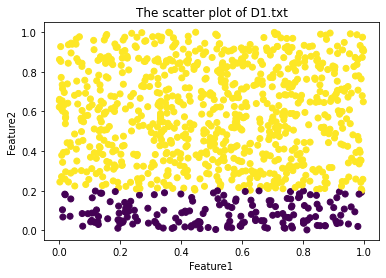
\includegraphics[width=0.5\textwidth]{images/q2_6a_D1.png}
        \caption{Scatter Plot of D1}
        \label{fig:q2_6a-d1}
    \end{figure}

      \begin{figure}[h!]
        \centering
        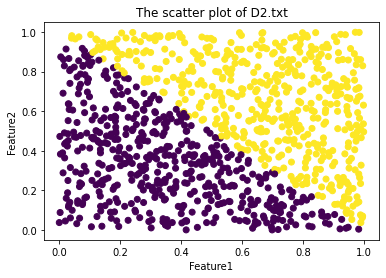
\includegraphics[width=0.5\textwidth]{images/q2_6a_D2.png}
        \caption{Scatter Plot of D2}
        \label{fig:q2_6a-d2}
    \end{figure}
  \end{soln}


    


  \item Visualize your decision tree's decision boundary (or decision region, or some other ways to clearly visualize how your decision tree will make decisions in the feature space).Then discuss why the size of your decision trees on D1 and D2 differ.  Relate this to the hypothesis space of our decision tree algorithm. \\
  \begin{soln}
      Using the data visualization, we can say that the decision boundaries of D1 and D2 are feature2=0.20 and feature2=-feature1+1, respectively. Their corresponding visualizations can be found in Figure \ref{fig:q2_6b-d1} and \ref{fig:q2_6b-d2}, respectively. The reason why D2's DT is much bigger is that the decision boundary of the data is non-horizontal/non-vertical. For D1, the decision boundary is horizontal, due to which the DT uses one node to make a decision on the label. On the other hand, there are multiple portions of D2 that have to be considered by DT in order to get the best fit of the decision boundary. Thus, D2's DT is more complex.

      \begin{figure}[h!]
        \centering
        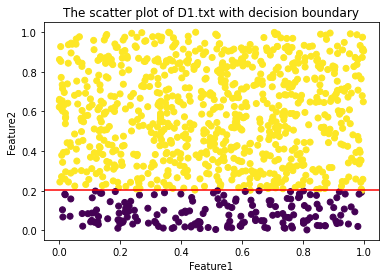
\includegraphics[width=0.5\textwidth]{images/q2_6b_D1.png}
        \caption{Scatter Plot of D1 with decision boundary}
        \label{fig:q2_6b-d1}
    \end{figure}

      \begin{figure}[h!]
        \centering
        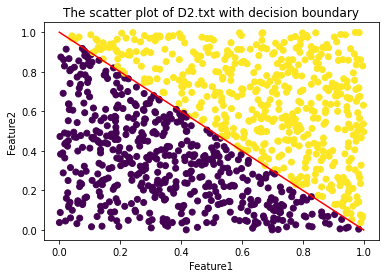
\includegraphics[width=0.5\textwidth]{images/q2_6b_D2.png}
        \caption{Scatter Plot of D2 with decision boundary}
        \label{fig:q2_6b-d2}
    \end{figure}
  \end{soln}


  \end{itemize}


\item (Learning curve)  [20 pts] We provide a data set Dbig.txt with 10000 labeled items.  Caution: Dbig.txt is sorted.
  \begin{itemize}
  
  \item You will randomly split Dbig.txt into a candidate training set of 8192 items and a test set (the rest).  Do this by generating a random permutation, and split at 8192.
  
  \item Generate a sequence of five nested training sets $D_{32} \subset D_{128} \subset D_{512} \subset D_{2048} \subset D_{8192}$ from the candidate training set.  The subscript $n$ in $D_n$ denotes training set size.  The easiest way is to take the first $n$ items from the (same) permutation above.  This sequence simulates the real world situation where you obtain more and more training data.
  
  \item For each $D_n$ above, train a decision tree.  Measure its test set error $err_n$.  Show three things in your answer: (1) List $n$, number of nodes in that tree, $err_n$. (2) Plot $n$ vs. $err_n$.  This is known as a learning curve (a single plot). (3) Visualize your decision trees' decision boundary (five plots). \\
  \end{itemize}
  \begin{soln}
      (1) Number of nodes is $D_{32}: 9, D_{128}: 31, D_{512}: 51, D_{2048}: 155, D_{8192}: 283$.\\
      Error on the test, $err_n$ is $D_{32}:  0.09236, D_{128}: 0.06028, D_{512}: 0.04480, D_{2048}: 0.03152, D_{8192}: 0.01382$

      (2) The $n$ vs $err_n$ plot is in Figure \ref{fig:q2-7}.\\
      
      \begin{figure}[h!]
        \centering
        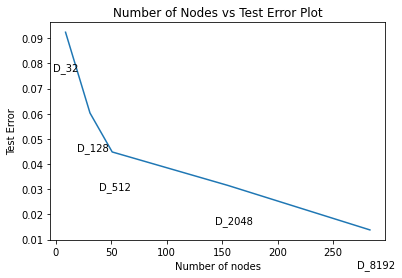
\includegraphics[width=0.5\textwidth]{images/q2_7_errorvsnode.png}
        \caption{Num of nodes vs Error Plot-My Decision Tree implementation}
        \label{fig:q2-7}
    \end{figure} \\
    (3) The scatter plots of my decision tree's decision boundaries can be found in Figures \ref{fig:q2_7_3a},\ref{fig:q2_7_3b},\ref{fig:q2_7_3c},\ref{fig:q2_7_3d},\ref{fig:q2_7_3e}

    \begin{figure}[h!]
        \centering
        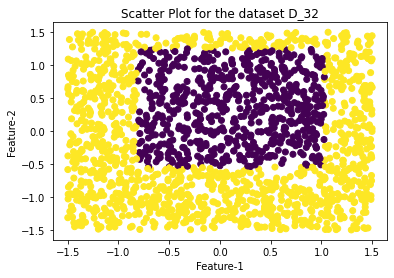
\includegraphics[width=0.5\textwidth]{images/q2_7_3a.png}
        \caption{Scatter of test set with decision boundary from D32's DT}
        \label{fig:q2_7_3a}
    \end{figure} \\
    \begin{figure}[h!]
        \centering
        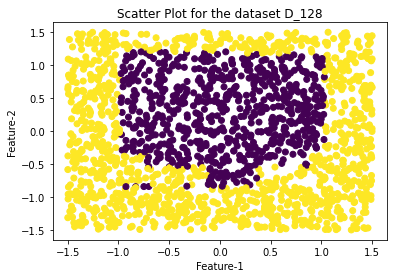
\includegraphics[width=0.5\textwidth]{images/q2_7_3b.png}
        \caption{Scatter of test set with decision boundary from D128's DT}
        \label{fig:q2_7_3b}
    \end{figure} \\
    \begin{figure}[h!]
        \centering
        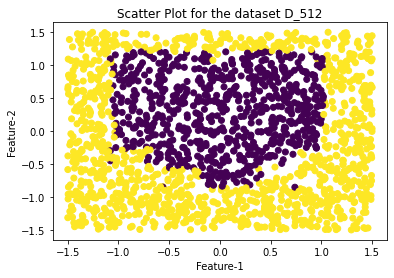
\includegraphics[width=0.5\textwidth]{images/q2_7_3c.png}
        \caption{Scatter of test set with decision boundary from D512's DT}
        \label{fig:q2_7_3c}
        
    \end{figure} \\

    \begin{figure}[h!]
        \centering
        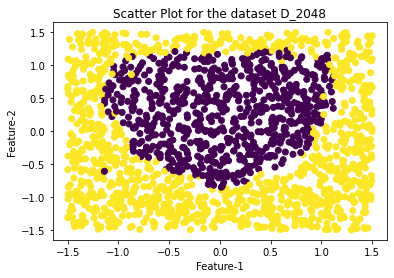
\includegraphics[width=0.5\textwidth]{images/q2_7_3d.png}
        \caption{Scatter of test set with decision boundary from D8192's DT}
        \label{fig:q2_7_3d}
    \end{figure} \\\

    \begin{figure}[h!]
        \centering
        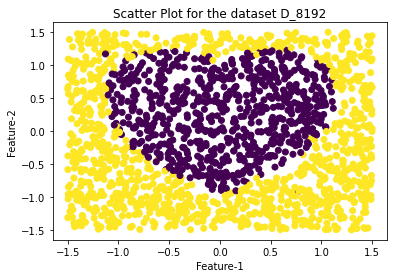
\includegraphics[width=0.5\textwidth]{images/q2_7_3e.png}
        \caption{Scatter of test set with decision boundary from D8192's DT}
        \label{fig:q2_7_3e}
    \end{figure} \\
  \end{soln}
\end{enumerate}

\section{sklearn [10 pts]}
Learn to use sklearn (\url{https://scikit-learn.org/stable/}).
Use sklearn.tree.DecisionTreeClassifier to produce trees for datasets $D_{32}, D_{128}, D_{512}, D_{2048}, D_{8192}$.  Show two things in your answer: (1) List $n$, number of nodes in that tree, $err_n$. (2) Plot $n$ vs. $err_n$.

\begin{soln}
(1)
    \begin{itemize}
        \item $n$, number of nodes is $D_{32}: 5, D_{128}: 27, D_{512}: 53, D_{2048}: 91, D_{8192}: 227$
        \item  $err_n$, error on the test set is $D_{32}: 0.2715, D_{128}: 0.0730, D_{512}: 0.0497, D_{2048}: 0.0376, D_{8192}: 0.0205$
    \end{itemize} \\
(2) Plot of $n$ vs. $err_n$ (Refer to Figure \ref{fig:q3nodeerror}).\\

\begin{figure}[h!]
        \centering
        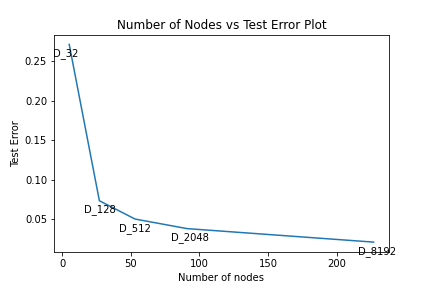
\includegraphics[width=0.5\textwidth]{images/q3_errorVsnode.png}
        \caption{Num of nodes vs test error-Sklearn Implementation}
        \label{fig:q3nodeerror}
    \end{figure}
\end{soln}

\section{Lagrange Interpolation [10 pts]}
Fix some interval $[a, b]$ and sample $n = 100$ points $x$ from this interval uniformly. Use these to build a training set consisting of $n$ pairs $(x, y)$ by setting function $y = sin(x)$. \\

Build a model $f$ by using Lagrange interpolation, check more details in \url{https://en.wikipedia.org/wiki/Lagrange_polynomial} and \url{https://docs.scipy.org/doc/scipy/reference/generated/scipy.interpolate.lagrange.html}. \\

Generate a test set using the same distribution as your test set. Compute and report the resulting model’s train and test error. What do you observe?
Repeat the experiment with zero-mean Gaussian noise $\epsilon$ added to $x$. Vary the standard deviation for $\epsilon$ and report your findings.

\begin{soln}
    The interval I chose was $[0,\pi]$ as sine is a periodic curve, and a polynomial function is not the best way to approximate the periodic nature of sine. Also, in this region, sine is always positive. \\

    I initially sampled 120 points from this range and assigned 100 to train and the rest to test, randomly. To estimate the performance of the Lagrange approximation of the original distribution, I used Mean Absolute Error(MAE). Like pointed out in one of the Piazza discussions, I noticed a very high MAE when I considered 100 points in the train set. The results were as follows: \\
    \begin{itemize}
        \item The mean absolute error on the train set is:5.766064785905992e+67
        \item The mean absolute error on the test set is:1.463716495501398e+68
    \end{itemize}
    
    One reason I could think of is, the scipy implementation of Lagrange interpolation always tries to find a (k-1) degree polynomial when given k points. This means that for a very small range like $[0,\pi]$, there will be a high-degree polynomial with very narrow peaks(local maximums and minimums). This leads to extremely high values of the values that weren't a part of the original train set.

    Thus, I chose to try the same with 15 points in the train set and 5 points in the test set. The results, in this case, were pretty accurate.
    \begin{itemize}
        \item The mean absolute error on the train set is:7.754835046246781e-05
        \item The mean absolute error on the test set is:6.44784521690478e-05
    \end{itemize}

The second part of the question requires us to add random gaussian noise to the train data with different standard deviations and observe the train and test errors. For this case, I considered the 100-sample training set and the 15-sample test set. I varied the standard deviation in multiples of $\pi$, i.e., 1/8, 1/4,1/2,3/4,1,2. I noticed that as the standard deviation increases, the MAE decreases for both the train and the test. Thus, adding the noise helps the Lagrange approximation to be closer to the original sine value.The observations were as follows:
\begin{itemize}
    \item The standard deviation considered is:0.39269908169872414 $=\pi/8$\\
The mean absolute error on the train set is:3.661584146300432e+69\\
The mean absolute error on the test set is:2.2564324196942475e+69\\
\item The standard deviation considered is:0.7853981633974483 $=\pi/4$\\
The mean absolute error on the train set is:4.9115168111289655e+72\\
The mean absolute error on the test set is:3.036625453439215e+72\\
\item The standard deviation considered is:1.5707963267948966 $=\pi/2$\\
The mean absolute error on the train set is:5.677339148170936e+47\\
The mean absolute error on the test set is:2.9233360288124813e+47\\
\item The standard deviation considered is:2.356194490192345 $=3\pi/4$\\
The mean absolute error on the train set is:2.8464381747818914e+31\\
The mean absolute error on the test set is:1.4801507856690453e+31\\
\item The standard deviation considered is:3.141592653589793 $=\pi$\\
The mean absolute error on the train set is:5765406851921.308\\
The mean absolute error on the test set is:3121671279758.343\\
\end{itemize}

However, the predictions are still not very accurate when considering the 15-sample case. The periodic nature of sine means some of these points get shifted to a region where the actual value of sine would be much different from the current values.

\end{soln}

\bibliographystyle{apalike}
\end{document}
